\section{Vertical Split Encoding for N-tuple Networks}

% 2048 の強いコンピュータプレイヤを作る最も成功した方法は,N タプルネットワークによる評価関数を強化学習によりチューニングするものである。Nタプルネットワークは,盤面の (局所的な) サンプリングとlook-up tableによる評価関数の近似関数である.各N-tupleに対して該当する場所の値をサンプリング・look-up tableから局所評価値を取得し,それら局所評価値を足し合わせることで全体の評価関数を得る.2048では,盤面の対称性から,一つのNタプルに対して8通りのサンプリングを行うことが一般的であり,本研究でもその対称性の利用を採用する.
The most successful approach to building a strong computer player for 2048 is to use an evaluation function based on N-tuple networks, whose parameters are tuned through reinforcement learning.
N-tuple networks are function approximators implemented with (local) sampling of the board and the corresponding lookup tables.
For each N-tuple (examples of N-tuples are given in Fig.~\ref{fig:NTupleVSE}), we sample a set of cells corresponding to the tuple elements, retrieve the corresponding values from the lookup table, and sum these values up to compute the overall evaluation value.
A common practice in 2048 is to perform eight-fold sampling for each N-tuple by exploiting board symmetries~\cite{SzJa14}, and does our study.

Increasing the size of the tuples is expected to yield significant performance improvements.
Oka and Matsuzaki~\cite{OkMa16} investigated the use of 6- and 7-tuples, showing that the use of 7-tuples achieved superior performance. We also confirmed for mini2048 (a $3\times 3$ variant of 2048) that increasing the size of N-tuples yielded a performance improvement of up to 6-tuples~\cite{TeMa25}.

% ニューラルネットワークと比べて,Nタプルネットワークは高速に評価値を計算することができるものの,一般に必要となるメモリ量が多い.盤面の各セルのとりうる値が $x$ 種類,タプルの数が m,タプルの大きさが n であるとき,look-up table は $m \times x^n$ 要素からなる.2048では,$\mbox{empty}, 2^1, 2^2, \ldots, 2^17$ の$x=18$通りの値をとりうるため,$n$ を増やしたときに必要となるメモリが問題となってしまう.実際,Jaskowski は,(multi-staging を採用できない)7タプルに拡大するよりも,6タプルとmulti-staging を組合せることが有用だと実験で示した.
However, N-tuple networks require a large amount of memory.
When we consider $m$ tuples of size $n$ and each cell on the board can have one of $x$ distinct values, a lookup table consists of $m \times x^n$ entries.
In 2048, since the number of possible cell values is 18 ($\mbox{empty}, 2^1, 2^2, \ldots, 2^{17}$), the memory requirement becomes an issue as $n$ increases.
Table~\ref{table:NTupleMemory} summarizes the number of parameters required in a lookup table for a single $n$-tuple and for eight $n$-tuples, when $n$ is between 6 and 9, as well as the memory usage when combining the currently dominant methods of multi-staging~\cite{YWHC16} and Temporal Coherence learning~\cite{Jask18}.
In practice, it has been believed that 7-tuples or larger could not work on commodity computers (e.g., within 64 GB of memory).
Indeed, Ja\'skowski~\cite{Jask18} experimentally demonstrated that it was more effective to use 6-tuples in combination with the multi-staging technique, rather than using a single 7-tuple without multi-staging.

% しかしながら,タプルサイズを増やすことができれば,大きな性能向上が見込まれる.Matsuzaki は,6タプルと7タプルの組合せとプレイヤの性能の関係を調べ,7タプルのほうが性能が優れていた.しかし,上述のメモリサイズの問題が発生する.
% Nタプルの大きさを 6~9 としたとき,1つのN-tuple に対してlook-up テーブルに必要となるパラメータ数,現在主流となっている Multi-staging と Temoral Coherence 学習を組み合わせた場合のメモリ量を表\ref{table:NTupleMemory}にまとめる.
% 一般は,4個以上のN-tuple を組み合わせて用いるので,commodity computer (e.g. computer with 64GB メモリ) では 7-tuple 以上を実現することができないと考えられていた.
\begin{table}
\setlength{\doublerulesep}{.4pt}
 \caption{Number of parameters and required memory size.  In the calculation of memory size, we assume an implementation of temporal coherence learning with 2 stages and 64 bits per element.}
\label{table:NTupleMemory}
 \centering\begin{tabular}{l|rr||l|rr}
\hline\hline
  \multicolumn{1}{c|}{network} & \multicolumn{1}{c}{parameters} & \multicolumn{1}{c||}{memory} & \multicolumn{1}{c|}{network} & \multicolumn{1}{c}{parameters} & \multicolumn{1}{c}{memory} \\
\hline
  $1 \times 6$-tuple & 34\,012\,224 & 1.5 GB &  $8 \times 6$-tuple & 272\,097\,792 & 12.2 GB \\
  $1 \times 7$-tuple & 612\,220\,032 & 27.4 GB &  $8 \times 7$-tuple & 4\,897\,760\,256 & ~~218.9 GB \\
  $1 \times 8$-tuple & 11\,019\,960\,576 & ~~492.6 GB &  $8 \times 8$-tuple & 88\,159\,684\,608 & 3.9 TB \\
  $1 \times 9$-tuple & 198\,359\,290\,368 & 8.9 TB &  $8 \times 9$-tuple & 1\,586\,874\,322\,944 & 70.9 TB \\
\hline
% (*    18 18 18 18 18 18 18 18 18 8)
% (/ (* 18 18 18 18 18 18 18 18 18 8 8 3 2) 1024.0 1024.0 1024.0)
 \end{tabular}
\end{table}

% このメモリサイズの問題を解決し,大規模タプルを効率的に扱うための新手法として,本研究では Vertical Split Encoding (VSE) を提案する.上述のとおり,メモリサイズがとても大きくなる理由は,盤面の取り得る値の種類 $x=18$ が大きいからである.一方で,著者らは2048における次の特徴に着目した.
% - 値の近いタイルの間の位置関係は重要である
% - 値の遠いタイルは相互作用しない
% - 空白マスの位置は重要である.
% これらの特徴のうち,2つ目の特徴から,ある値のタイルに着目すると,それと値が大きく離れたタイルは区別する必要がないことを示唆する.例えば,値が 2 (= $2^1$) のタイルに着目すると,その周辺にある値 $2048 = 2^{11}$ や $4096 = 2^{12}$ を区別するのはほとんど意味をなささい.したがって,そのような値が大きく離れたタイルを同一視することで,パラメータ数を減らすことができると考えた.

To address the issue of memory requirement and hence to enable large N-tuple networks, this study proposes a novel method called \emph{Vertical Split Encoding} (VSE)~\footnote{The idea behind the term ``Vertical'': the input space of 2048 is in three dimensions, the first two are for the position on a board, and the third is for the cell values. Vertical Split Encoding works on this third dimension.}.
As noted above, the main reason for the huge memory requirement is that the number of possible cell values on the board is large, $x = 18$.
Here, we notice the following characteristics of 2048.
\begin{itemize}
 \item The relative positions of tiles with \emph{similar} values are important.
 \item Tiles with \emph{widely different} values do not interact.
 \item The positions of empty cells are important.
\end{itemize}
Among these, the second characteristic suggests that, when looking at a particular tile value, it is unnecessary to distinguish tiles whose values are very far apart. For example, when looking at a tile of value $2^1$, distinguishing whether the neighboring tiles are $2^{11}$ or $2^{12}$ is almost meaningless.
Therefore, by equating tiles with widely different values, we can reduce the number of possible values and accordingly the number of parameters in the lookup tables.

% この考えに基づき,Vertical Split Encoding は,盤面を,いくつかの値を同一視した複数の盤面にエンコードする.
% 各エンコードでは,着目したい値の範囲を value range とし,その範囲より小さい・大きい値はすべて S・L に置き換える.
% ただし,上で述べた2048の特徴の3より,empty cell (E) については特別扱いする.
% 図に具体例を示す.ここでは,value ranges は 1--10 と 11-17 とする.
% このとき,一つ目のエンコードでは,$2^{11}$~$2^{17}$の値を持つタイルはすべて L となり,2つ目のエンコードでは
% $2^{1}$~$2^{10}$ のタイルはすべて S となる.これにより,1つ目のエンコードについては,各セルのとりうる値が $x_1 = 1 + 10 + 1 = 12$ 通り,2つ目のエンコーディングでは $x_2 = 1 + 1 + 7 = 9$ 通りとなり,look-up table の要素数を大きく減少させられる.
Based on this idea, Vertical Split Encoding maps a board into multiple board instances, in each of which some board cells have the same label.
First, we define a set of \emph{value ranges} of interest: All values smaller than this range are replaced by $S$, and all the larger values are replaced by $L$.
To address the third characteristic mentioned above, we treat empty cells (E) separately.

A concrete example is shown in Fig.~\ref{fig:VSE-example}, where value ranges of interest are $2^1$--$2^8$ and $2^9$--$2^{17}$.
In the first mapping, all tiles with values larger than $2^{8}$ are replaced by $L$.
In the second mapping, all the tiles with values smaller than $2^{9}$ are replaced by $S$.
After these mappings, the resulting possible values are $[{E}, 2^1, 2^2, 2^3, 2^4, 2^5, 2^6, 2^7, 2^8, {L}]$ in the first mapping and $[{E}, {S}, 2^9, 2^{10}, 2^{11}, 2^{12}, $\break$2^{13}, 2^{14}, 2^{15}, 2^{16}, 2^{17}]$ in the second mapping.
As a result, the numbers of possible values are $x_1 = 10$ and $x_2 = 11$, respectively, which significantly reduces the memory requirement for the lookup tables.

\begin{figure}
 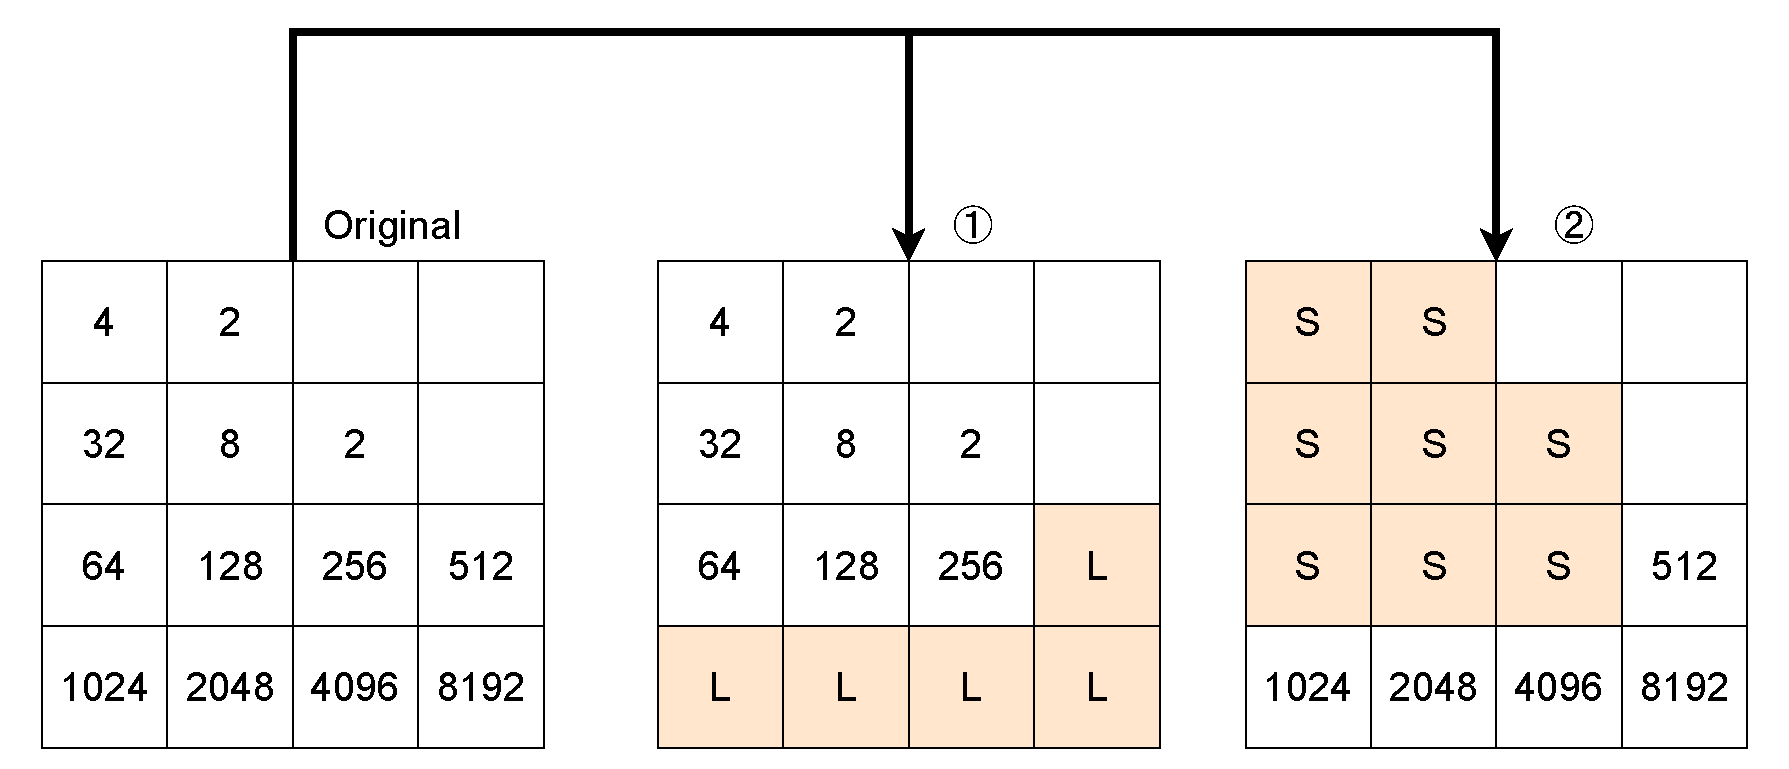
\includegraphics[width=.9\linewidth]{figures/VSE-example.pdf}
 \caption{An example of Vertical Split Encoding with two value ranges 1--8 and 9--17.}
 \label{fig:VSE-example}
\end{figure}

% 後述する2048に対する実験では,7タプル,8タプル,9タプルに対し,それぞれ,2つ,3つ,4つのvalue ranges からなるVSEを適用し,プレイヤの性能を評価する.

We can extend the idea to $k$-VSE, with $k$ value ranges of interest.
In the experiments on 2048 described later, we apply 2-, 3-, and 4-VSE.

% LocalWords:  approximators Ja skowski VSE
